\section{new section}\label{new-section}

\begin{itemize}
\itemsep1pt\parskip0pt\parsep0pt
\item
  item

  \begin{itemize}
  \itemsep1pt\parskip0pt\parsep0pt
  \item
    item 1.1
  \item
    item 1.2
  \item
    new item
  \end{itemize}
\end{itemize}

\begin{align}
x_i &= y_i \label{eq:tmp1}\\
x_i + y_i &= y_i
\end{align}

cite me: \textcite{Abb97}

Reference math: \eqref{eq:tmp1}

Math without numbering:

\begin{align*}
x_i &= y_i \\
x_i + y_i &= y_i
\end{align*}

\begin{Shaded}
\begin{Highlighting}[]
\NormalTok{x <-}\StringTok{ }\DecValTok{1}
\end{Highlighting}
\end{Shaded}

\begin{Shaded}
\begin{Highlighting}[]
\KeywordTok{ggplot}\NormalTok{(}\KeywordTok{data.frame}\NormalTok{(}\DataTypeTok{x =} \DecValTok{1}\NormalTok{:}\DecValTok{10}\NormalTok{, }\DataTypeTok{y =} \DecValTok{11}\NormalTok{:}\DecValTok{20}\NormalTok{)) +}\StringTok{ }
\StringTok{  }\KeywordTok{geom_point}\NormalTok{(}\KeywordTok{aes}\NormalTok{(x, y)) +}\StringTok{ }
\StringTok{  }\KeywordTok{theme_thesis}\NormalTok{()}
\end{Highlighting}
\end{Shaded}

\begin{figure}[htbp]
\centering
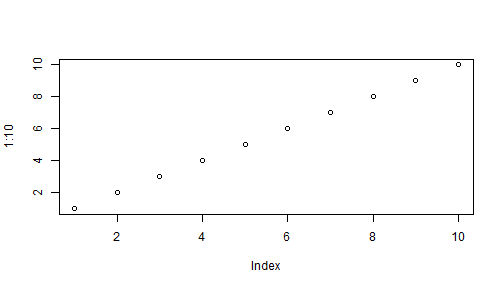
\includegraphics{figs/test/unnamed-chunk-2-1.png}
\caption{plot of chunk unnamed-chunk-2}
\end{figure}
